\chapter{Introducción específica} % Main chapter title

\label{Chapter2}

En este capítulo se detallan las tecnologías aplicadas en el desarrollo del trabajo, destacando los componentes de inteligencia artificial seleccionados para la detección y seguimiento de personas. Finalmente se describe los desafíos que el sistema debe superar para alcanzar los requerimientos establecidos.

%----------------------------------------------------------------------------------------
%	SECTION 1
%----------------------------------------------------------------------------------------

\section{Requerimientos}
\label{sec:requerimientos}

En esta sección se detallan los requerimientos establecidos para este trabajo, que guiaron el diseño y la implementación del mismo:

\begin{enumerate}
\item Requerimientos asociados con el proceso de inteligencia artificial:
	\begin{enumerate}
	\item Detectar y seguir personas en un video, excluir otros elementos.
	\item Generar características que permitan luego re-identificar personas perdidas.
	\item Resolver problemáticas en el seguimiento de las personas utilizando sus características.
	\end{enumerate}
\item Requerimientos asociados con la interfaz de usuario:
	\begin{enumerate}
	\item Mediante una interfaz web poder definir las zonas de interés.
	\item Medir el comportamiento de cada persona con las zonas de interés.
	\item Poder observar en tiempo real las métricas obtenidas por el sistema.
	\end{enumerate}
\item Requerimientos asociados con el sistema de monitoreo:
\begin{enumerate}
	\item Se considerará que una persona es correctamente monitoreada si al menos se mantuvo su seguimiento el 80\% del tiempo que circuló en el recinto.
	\item Se considerará que el sistema funciona dentro de los parámetros aceptables si entre el 80\% y 100\% de las personas en el video fueron correctamente monitoreadas.
	\end{enumerate}
\item Requerimientos asociados con regulaciones:
\begin{enumerate}
	\item Los videos utilizados no inflijan derechos de privacidad.
	\item El sistema no asociará las personas en seguimiento con un persona física real.
	\end{enumerate}
\end{enumerate}

\newpage

%----------------------------------------------------------------------------------------
%	SECTION 2
%----------------------------------------------------------------------------------------

\section{Modelos de inteligencia artificial utilizados}
\label{sec:modelosIA}

En esta sección se realiza una introducción a los modelos de inteligencia artificial utilizados. En la sección \ref{sec:cadenaProcesamiento} se detalla la implementación e integración de los mismos.

\subsection{Detector Yolo}

\textit{Yolo (You Only Look once)} es un modelo de inteligencia artificial que utiliza aprendizaje profundo y redes convolucionales para detectar objetos en imágenes. El nombre del modelo hace referencia a su arquitectura, ya que permite detectar múltiples objetos de una imagen con solo procesarla una vez (solo ``verla'' una vez). El proceso de detección está conformado por los siguientes pasos:

\begin{itemize}
\item Se divide la imagen original en una cuadrícula de ``SxS''.
\item En cada celda se predicen ``N'' detecciones y se calcula la precisión de detección de cada una.
\item Una detección se conforma por una caja que la situá en la imagen original (coordenadas X e Y, alto y ancho). Esta caja se la conoce como \textit{bounding boxe (bboxe)}.
\item Las detecciones duplicadas o que posean un baja precisión de detección (configurable por el usuario) son descartadas.
\end{itemize}

En la figura \ref{fig:diagramaYolo} se observa un ejemplo del proceso completo de detección, en el cual el sistema detecta tres objetos en la imagen: un perro, una bicicleta y un auto. El resultado de procesar esta imagen por Yolo son tres bboxes con las coordenadas y la precisión de detección de cada objeto.

\begin{figure}[ht]
	\centering
	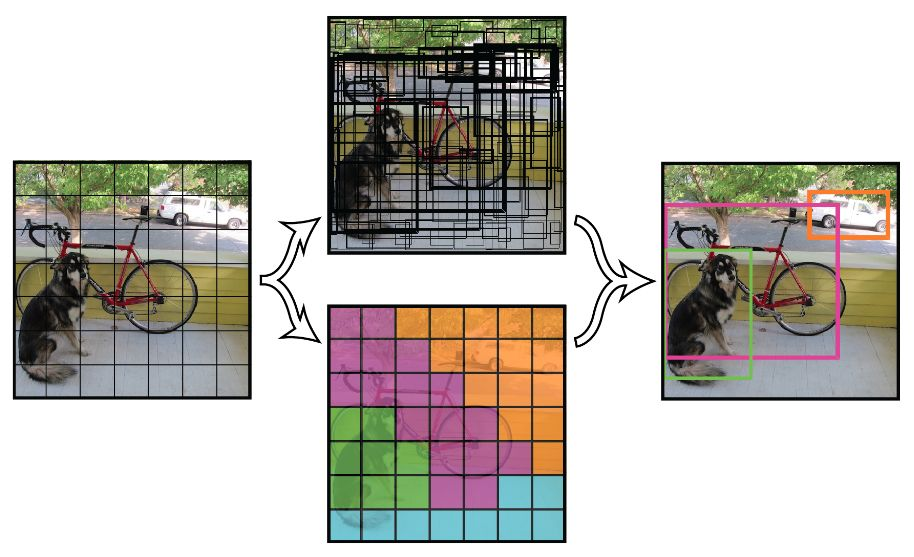
\includegraphics[scale=.60]{./Figures/yolo.jpg}
	\caption{Esquema de funcionamiento de Yolo\protect\footnotemark.}
	\label{fig:diagramaYolo}
\end{figure}

\footnotetext{Imagen tomada de \url{https://pjreddie.com/darknet/yolov1/}}

\newpage

Otros modelos utilizados para detectar objetos en imágenes son los derivados de las arquitecturas ``R-CNN'' y ``Fast R-CNN'' \citep{RCNN}, que se basan en dividir la imagen en múltiples regiones y por cada una de ellas efectuar una clásica clasificación de imágenes. El proceso de dividir la imagen en regiones se encuentra bastante optimizado en las últimas versiones de estas arquitecturas, pero el sistema aplica una clasificación de imágenes por cada región candidata. Los modelos derivados de estas arquitecturas son más lentos que Yolo (no recomendables para procesos en tiempo real) pero son más precisos, como se ilustra en la tabla \ref{tab:comparativaDetectores}.

\begin{table}[h]
	\centering
	\caption[Comparativa de detectores]{Comparativa de detectores.}
	\begin{tabular}{l c c}    
		\toprule
		\textbf{Detector}   & \textbf{Velocidad [FPS]} & \textbf{Precisión promedio [\%]} \\
		\midrule
		R-CNN & 0,02 & 58,5\% \\
		Fast R-CNN & 0,5 & 70\% \\
		Faster R-CNN & 7 & 73,2\% \\
		Yolo & 45 & 63,4\% \\
		\bottomrule
		\hline
	\end{tabular}
	\label{tab:comparativaDetectores}
\end{table}

La velocidad de ejecución de un modelo de inteligencia artificial se mide en \textit{frames per seconds (FPS)}, es decir, a que velocidad se pueden procesar imágenes de forma consecutiva sin presentar un retraso en el video generado de salida.

\subsection{Seguidor Deepsort}

\textit{Deepsort (Deep Simple Online Tracking)} es un modelo de inteligencia artificial que utiliza aprendizaje profundo y técnicas de visión por computadora para seguir múltiples objetos en imágenes. El modelo Deepsort es la evolución del modelo seguidor ``Sort'', que incorpora un comparador de imágenes o características al sistema junto al filtro de Kalman \citep{KALMAN_FILTER}, para asociar las detecciones en cada frame. En la figura \ref{fig:deepsortArq} se observa un diagrama de alto nivel de la arquitectura Deepsort.

\begin{figure}[ht]
	\centering
	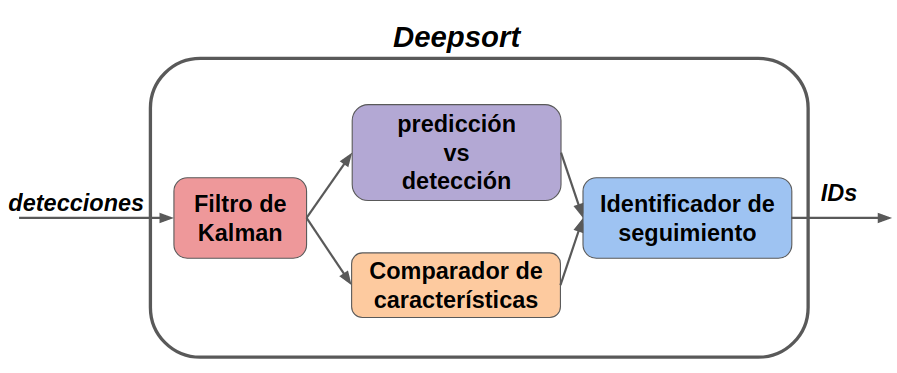
\includegraphics[scale=.55]{./Figures/deepsort.png}
	\caption{Arquitectura de Deepsort.}
	\label{fig:deepsortArq}
\end{figure}

El seguidor consume a la entrada las detecciones en forma de bboxes que arroja el detector, como resultado retorna las bboxes con los identificadores de seguimiento asociados a las detecciones.

\newpage

En la figura \ref{fig:deepsortProcess} se ilustra el proceso de seguimiento, el cual esta conformado por los siguientes pasos:
\begin{itemize}
\item Por cada detección que ingresa al seguidor, se estima la próxima posición de cada bboxe utilizando el filtro de Kalman. Este filtro estima la posición nueva utilizando la dinámica de movimiento que representa al objecto en seguimiento, en este caso, la dinámica de movimiento de personas.
\item En el siguiente frame se asocian las nuevas detecciones con las predicciones calculadas. Aquellas bboxes que coincidan con las predicciones por arriba de un margen configurable se las asocia al mismo objecto. Cada objecto identificado por el seguidor obtiene un identificador único de seguimiento (ID).
\item Aquellas bboxes que no coincidan con las predicciones se buscará asociarlas con detecciones anteriores utilizando el comparador de imágenes o características. Este sistema robustece al proceso cuando un objecto desaparece algunos frames de la imagen, permitiendo al sistema re-encontrar objectos en seguimiento que no hayan estado disponibles en todos los frames de forma continua.
\end{itemize}

\begin{figure}[ht]
	\centering
	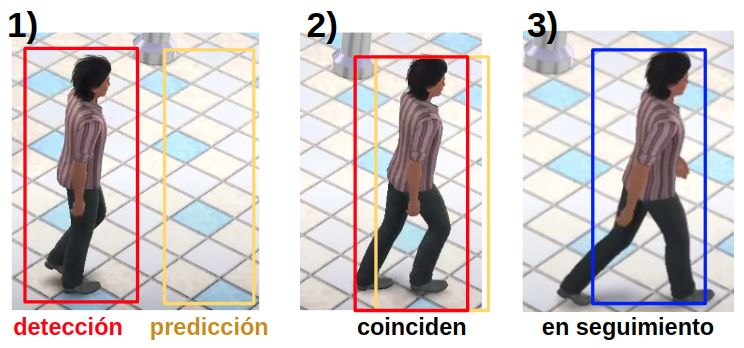
\includegraphics[scale=.65]{./Figures/deepsortProcess.jpg}
	\caption{Esquema de funcionamiento de Deepsort.}
	\label{fig:deepsortProcess}
\end{figure}

La principal ventaja de Deepsort es que gracias al comparador de características es más robusto a oclusiones o pérdidas de detección momentáneas, además de ser uno de los modelos seguidores de objectos más rápidos. En la tabla \ref{tab:comparativaSeguidores} se comparan distintos modelos seguidores de objectos.

\begin{table}[h]
	\centering
	\caption[Comparativa de seguidores]{Comparativa de seguidores.}
	\begin{tabular}{l c c c}    
		\toprule
		\textbf{Seguidor} & \textbf{Velocidad [FPS]}  & \textbf{Precisión [MOTA]} & \textbf{Intercambios de IDs} \\
		\midrule
		POI & 10 & 61,4\% & 805 \\
		Sort & 60 & 59,8\% & 1423 \\
		Deepsort & 40 & 66,1\% & 781 \\
		\bottomrule
		\hline
	\end{tabular}
	\label{tab:comparativaSeguidores}
\end{table}

\newpage

\subsection{Extractor de características Osnet}
\label{sec:exactorOsnet}

\textit{Osnet (Omni-Scale Network)} \citep{OSNET} es un modelo de inteligencia artificial que utiliza aprendizaje profundo y redes convolucionales para extraer vectores de características de una imagen. El nombre del modelo hace referencia a su arquitectura, ya que permite detectar tanto características globales (entorno) como características locales (detalles). En la figura \ref{fig:osnet} se observa un diagrama de alto nivel de la arquitectura Osnet.

\begin{figure}[ht]
	\centering
	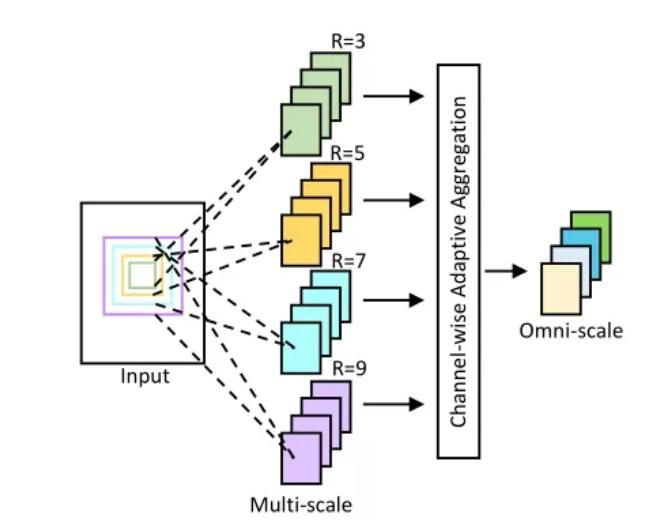
\includegraphics[scale=.60]{./Figures/osnet.jpg}
	\caption{Esquema de funcionamiento de Osnet\protect\footnotemark.}
	\label{fig:osnet}
\end{figure}

\footnotetext{Imagen tomada de \url{https://www.programmersought.com/article/12063493294/}}

El extractor consume a la entrada las imágenes en forma de bboxes que arroja el detector o el seguidor, como resultado retorna un vectores de 512 dimensiones por cada imagen. Cada vector representa las características globales y locales (omni) detectadas de cada persona. En la figura \ref{fig:osnetFeatureMap} se observa un ejemplo de los patrones o características que Osnet observa y traduce a un vector numérico de datos.

\begin{figure}[ht]
	\centering
	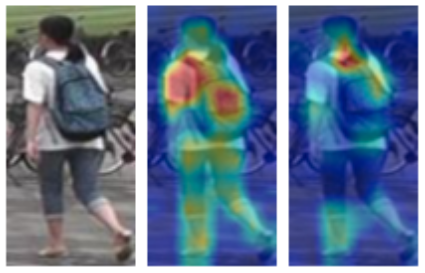
\includegraphics[scale=.60]{./Figures/osnetFeatureMap.png}
	\caption{Características que Osnet observa de una persona\protect\footnotemark.}
	\label{fig:osnetFeatureMap}
\end{figure}

\footnotetext{Imagen tomada de \url{https://kaiyangzhou.github.io/deep-person-reid/user_guide.html}}

\newpage

Existen otros modelos de inteligencia artificial que se utilizan para extraer características de personas. Un modelo muy popular es \textit{DeepMar (Multi-attribute Recognition)} \citep{DEEPMAR}, que extrae una serie de atributos relativos a la persona y su vestimenta. En la figura \ref{fig:deepmar} se observa un ejemplo de los atributos que extrae DeepMar de una persona.

\begin{figure}[ht]
	\centering
	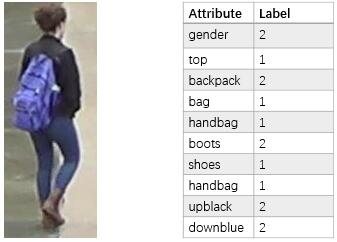
\includegraphics[scale=.8]{./Figures/deepmar.png}
	\caption{Atributos que DeepMar observa de una persona\protect\footnotemark.}
	\label{fig:deepmar}
\end{figure}

\footnotetext{Imagen tomada de \url{https://github.com/sxzrt/DukeMTMC-reID_evaluation}}

La ventaja de Osnet respecto a otros modelos como DeepMar es que sus vectores son más representativos, caracterizando mejor a las personas. Osnet es muy robusto obteniendo características que permiten diferenciar a dos personas muy similares, como se observa en la figura \ref{fig:osnetDosPersonas}.

\begin{figure}[ht]
	\centering
	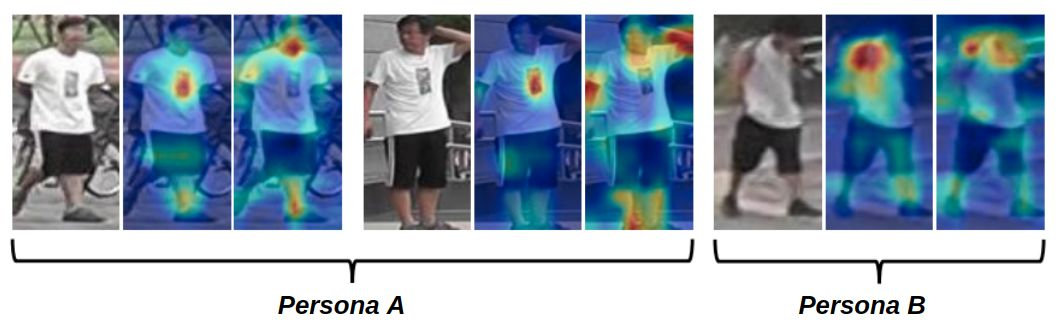
\includegraphics[scale=0.5]{./Figures/osnetDosPersonas.jpg}
	\caption{Características de Osnet sobre dos personas similares\protect\footnotemark.}
	\label{fig:osnetDosPersonas}
\end{figure}

\footnotetext{Imagen tomada de \url{https://arxiv.org/pdf/1905.00953.pdf}}

En la tabla \ref{tab:comparativaExtractores} se comparan distintos modelos extractores de características de personas.

\begin{table}[h]
	\centering
	\caption[Comparativa de extractores de características]{Comparativa de extractores de características.}
	\begin{tabular}{l c c}    
		\toprule
		\textbf{Extractor} & \textbf{Exactitud [\%]}  & \textbf{Precisión [\%]} \\
		\midrule
		DeepMar & 70,4\% & 82,2\% \\
		HydraPlusNet & 72,2\% & 83,0\% \\
		Osnet & 76,0\% & 88,3\% \\
		\bottomrule
		\hline
	\end{tabular}
	\label{tab:comparativaExtractores}
\end{table}

\newpage

%----------------------------------------------------------------------------------------
%	SECTION 3
%----------------------------------------------------------------------------------------

\section{Agrupación de datos (clustering)}
\label{sec:clustering}

La agrupación de datos \textit{(clustering)} es el proceso que permite establecer relaciones entre elementos que poseen características en común conformando grupos de datos. De ahora en adelante se hará mención a estos grupos de datos bajo el nombre de \textit{clusters}. Los clusters representan a los datos que los componen  unidos por sus características o patrones que comparten.

Cada cluster contará con un hipotético punto intermedio (el centroide) que se irá modificando con la entrada o salida de datos al grupo. El clustering alcanzará el equilibrio cuando exista una coincidencia entre el hipotético punto de valor intermedio dentro del grupo y su relación con sus elementos. 

En la figura \ref{fig:clusterDigitos} se observa un ejemplo de clustering de imágenes de digitos, en el cual, cada cluster está representado por un color y conformado por el dígito que lo caracteriza.

\begin{figure}[ht]
	\centering
	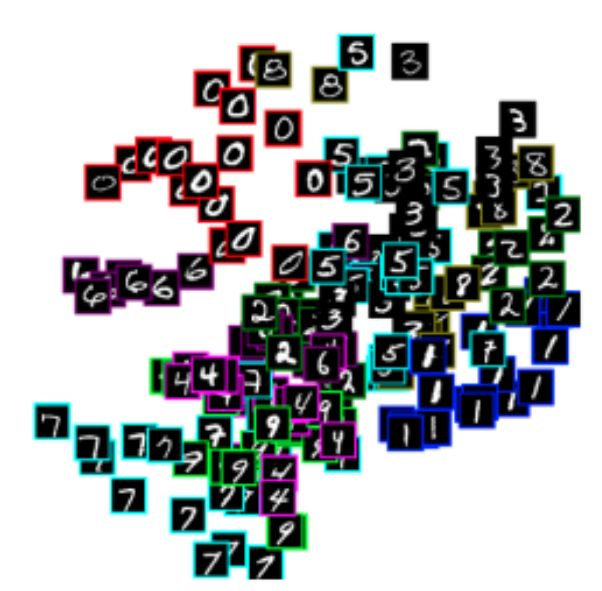
\includegraphics[scale=0.7]{./Figures/clusterDigitos.jpg}
	\caption{Ejemplo de clusters de dígitos.}
	\label{fig:clusterDigitos}
\end{figure}

En la sección \ref{sec:segmentacionPersonas} se detalla la implementación de esta técnica para la segmentación y re-identificación de personas.

\newpage

%----------------------------------------------------------------------------------------
%	SECTION 4
%----------------------------------------------------------------------------------------

\section{Desafíos en el seguimiento de personas}
\label{sec:desafiosSeguimiento}

Las desafíos que se detallan en esta sección son problemáticas generales a la hora de seguir un objeto con el mismo identificador, todo el tiempo que este permanece visible en escena. Uno de los objetivos del sistema es detectar estos casos, a fin de recuperar o re-asignar correctamente el identificador de cada persona en monitoreo. 

Mantener el mismo identificador en el seguimiento de personas es más complejo, debido que las personas en movimiento son caóticas: forman y disuelven grupos de personas, cambian su pose constantemente, pueden salir y volver de escena, etc. En la sección \ref{sec:oclusionesReID} se detallan las técnicas empleadas de manejo de oclusiones y re-identificación de personas que resuelven estos desafíos.

\subsection{Pérdida de identificador}

La pérdida del identificador de seguimiento (ID) de una persona en monitoreo generalmente ocurre cuando esta pasa por detrás de otro objecto que la ocluye. El objecto que la ocluye puede ser estático (un mueble, un cartel, etc) o dinámico (otra persona o grupo de personas en la escena).

En la figura \ref{fig:id_lost} se observa un ejemplo de pérdida de ID cuando un sujeto azul pasa por detrás de un sujeto verde. Cuando el individuo vuelve a ser detectado por el seguidor al concluir la oclusión, el sistema confunde a esta persona con una nueva detección, asignado un identificador nuevo (persona roja). De esta forma, el identificador azul se perdió del sistema y se generó un nuevo erróneamente.

\begin{figure}[!htpb]
     \centering
     \begin{subfigure}[b]{0.3\textwidth}
         \centering
         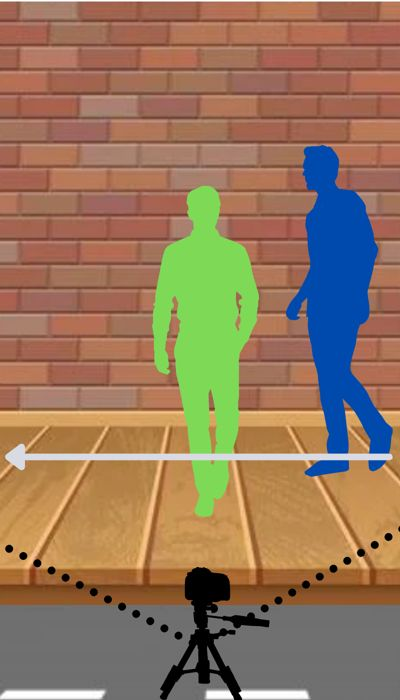
\includegraphics[width=.65\textwidth]{./Figures/id_lost1.jpg}
         \caption{Dos personas en escena.}
         \label{fig:id_lost1de3}
     \end{subfigure}
     \hfill
     \begin{subfigure}[b]{0.3\textwidth}
         \centering
         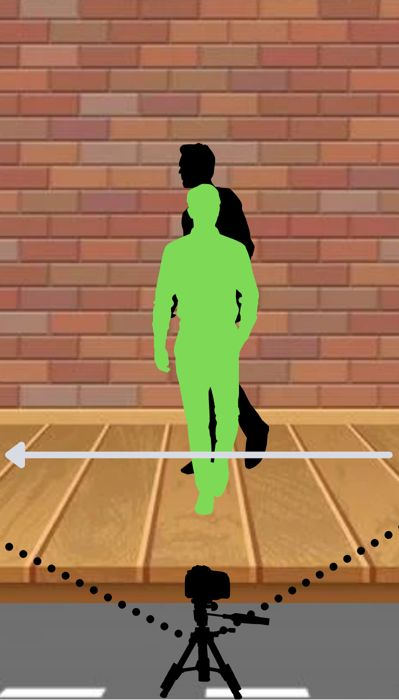
\includegraphics[width=.65\textwidth]{./Figures/id_lost2.jpg}
         \caption{Oclusión.}
         \label{fig:id_lost2de3}
     \end{subfigure}
     \hfill
     \begin{subfigure}[b]{0.3\textwidth}
         \centering
         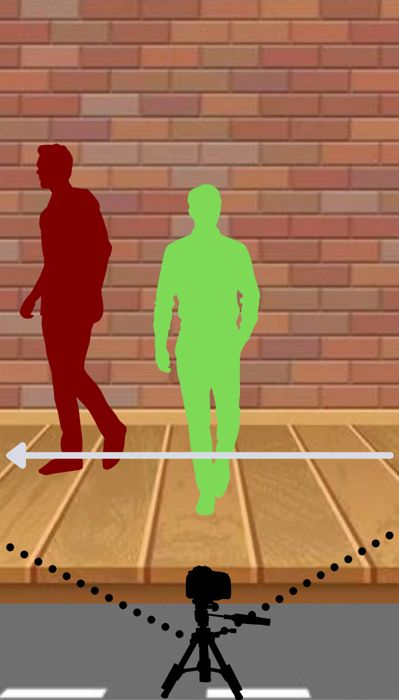
\includegraphics[width=.65\textwidth]{./Figures/id_lost3.jpg}
         \caption{Pérdida del identificador.}
         \label{fig:id_lost3de3}
     \end{subfigure}
        \caption{Ejemplo de pérdida del identificador azul.}
        \label{fig:id_lost}
\end{figure}

\newpage

\subsection{Intercambio de identificador}

El intercambio del identificador de seguimiento (ID) de una persona en monitoreo generalmente ocurre cuando dos personas se cruzan en movimiento. Al momento que ambas personas se cruzan, sus bboxes poseen una ubicación geométrica y un vector de movimiento similar. Estos factores producen que el filtro de Kalman del seguidor no pueda diferenciar las detecciones, y recae toda la responsabilidad en el extractor de características del mismo en diferenciarlas. En general, el seguidor Deepsort no es lo suficientemente robusto para resolver esta situación.

En la figura \ref{fig:id_switch} se observa un ejemplo de intercambio de ID cuando un sujeto azul se cruza con un sujeto rojo en movimiento. Cuando los individuos vuelven a ser detectados por el seguidor al concluir la oclusión, el sistema confunde a estas personas mezclando sus identificadores. De esta forma, el identificador azul se asigna a la persona que antes era roja, y el identificador rojo se asigna a la persona que antes era azul.

\begin{figure}[!htpb]
     \centering
     \begin{subfigure}[b]{0.3\textwidth}
         \centering
         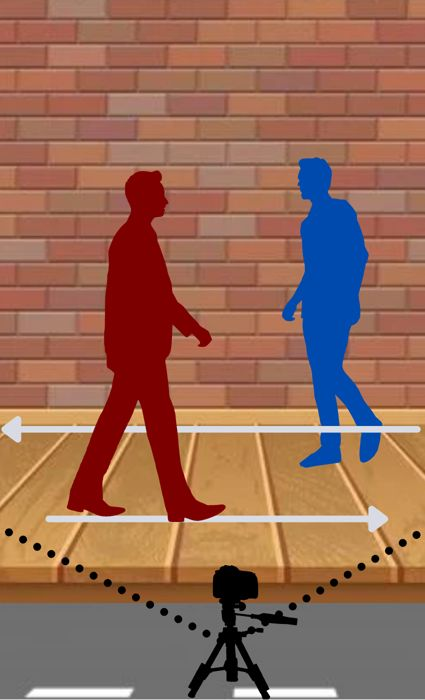
\includegraphics[width=.65\textwidth]{./Figures/id_switch1.jpg}
         \caption{Dos personas en escena.}
         \label{fig:id_switch1de3}
     \end{subfigure}
     \hfill
     \begin{subfigure}[b]{0.3\textwidth}
         \centering
         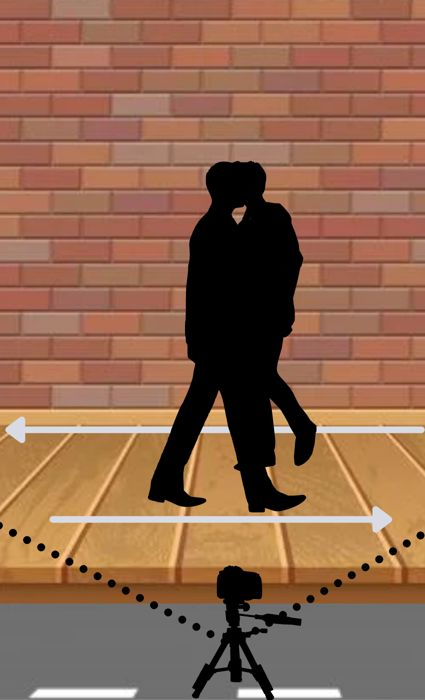
\includegraphics[width=.65\textwidth]{./Figures/id_switch2.jpg}
         \caption{Oclusión mutua.}
         \label{fig:id_switch2de3}
     \end{subfigure}
     \hfill
     \begin{subfigure}[b]{0.3\textwidth}
         \centering
         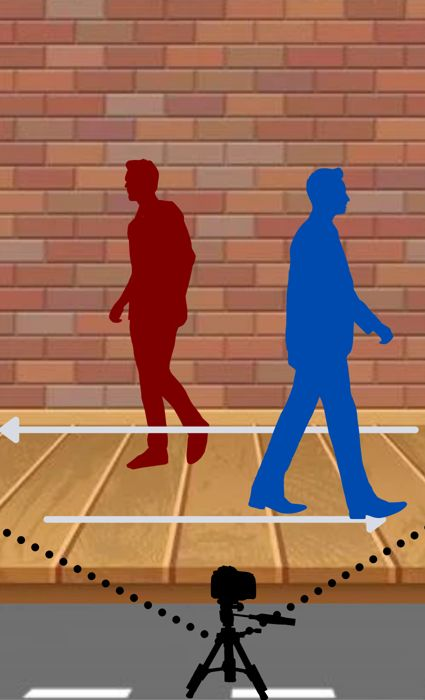
\includegraphics[width=.65\textwidth]{./Figures/id_switch3.jpg}
         \caption{Intercambio de colores.}
         \label{fig:id_switch3de3}
     \end{subfigure}
        \caption{Ejemplo de intercambio de identificador entre personas.}
        \label{fig:id_switch}
\end{figure}

\newpage
%----------------------------------------------------------------------------------------
%	SECTION 5
%----------------------------------------------------------------------------------------

\section{Zonas de interés}
\label{sec:zonasInteres}

Una zona de interés es un área en el espacio limitada por un polígono dibujado en el piso, diferenciadas por colores o nombres. Estas zonas se utilizan para identificar escenarios, datos o cualquier particularidad que el usuario desea obtener de esa región. El sistema detecta toda persona que ingrese en las zonas, contabilizando el tiempo de permanencia, su actividad e identificando a los individuos con el color de la zona a la que pertenecen.

En la figura \ref{fig:zonasInteres} se observa un ejemplo de un espacio delimitado por tres zonas de interés: el área de retiro de efectivo o pago (zona azul), el área de bebidas o barra (zona roja) y la zona que delimita el espacio observable del bar (zona verde).

\begin{figure}[ht]
	\centering
	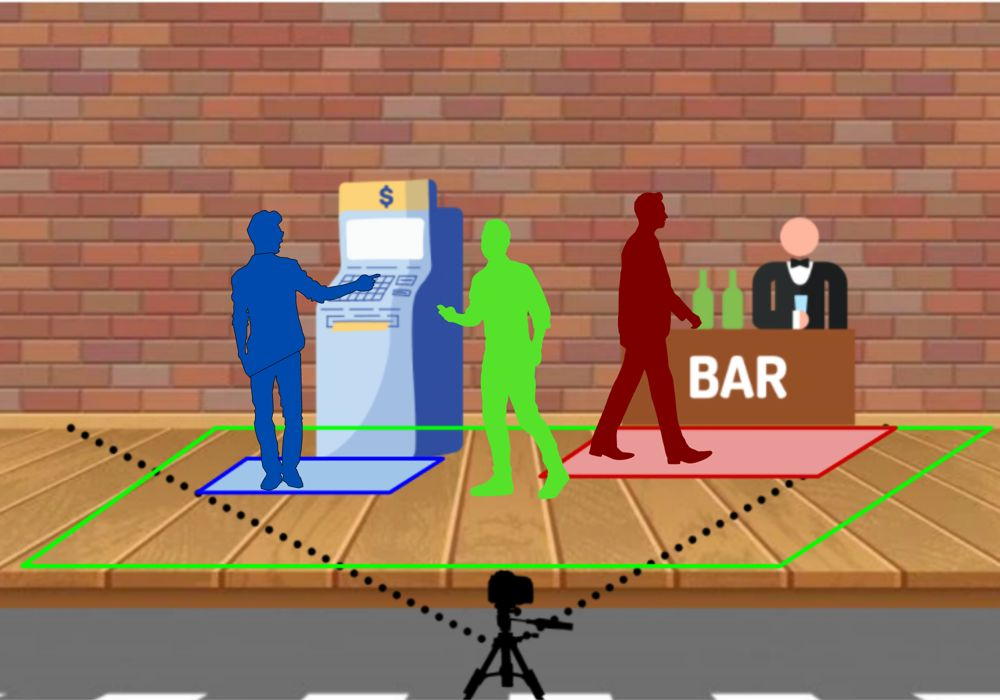
\includegraphics[scale=1.2]{./Figures/zonasInteres.jpg}
	\caption{Ejemplo de zonas de interés.}
	\label{fig:zonasInteres}
\end{figure}

En la sección \ref{sec:definicionZonasInteres} se detalla como el usuario puede crear las zonas de interés con la interfaz del sistema.